%brauche folgende pakete
%\usepackage{tikz}
%\usetikzlibrary{circuits.ee.IEC}
%\usepackage{placeins}






\chapter{Arbeitspaket Simulation}
Für Analyse, Entwurf und Implementierung dieses Arbeitspakets übernahm Herr Welker die Verantwortung.


\section{Analysephase I - Verwendung existierender Bausteine}
Gemäß Projektspezifikation wurde gewünscht, dass die zu entwickelnde Simulation in Echtzeit laufen soll (1 Sekunde Simulation soll einer Sekunde in der Realität entsprechen), so dass die Simulationsergebnisse später ggf. mit dem realen Versuchsaufbau verglichen oder gar verbunden werden können. 

Zunächst wurde hierzu der Einsatz eines \textit{Rapid Prototyping System} von dSPACE erwogen. %https://de.mathworks.com/products/connections/product_detail/product_35337.html
Das Problem hierbei ist jedoch die Beschaffung (Hardware) und der nach bereits früher erhaltenen Aussagen extrem hohe Preis. 

Eine weitere Alternative wäre \textit{Simulink Desktop Real-Time}. %https://de.mathworks.com/products/simulink-desktop-real-time.html
Hier wird zwar keine kostspielige externe Hardware benötigt, aber auch die Anschaffungskosten von 2000 Euro %https://de.mathworks.com/pricing-licensing.html?prodcode=WT
wären für den Simulationsteil des Projekts wesentlich zu hoch. 

Aufgrund dieser Randbedingungen wurde von einer Simulation in Echtzeit zunächst wieder Abstand genommen.

Ein zusätzliches Ziel der Simulation sollte eine Kommunikations-Verbindung mit der GUI sein. Hierbei wäre es wünschenswert, wenn die Kommunikation äquivalent zur echten Hardware funktionieren würde, so dass mit ein- und derselben GUI sowohl Simulation als realer Versuchsaufbau angesprochen werden können. 

Da im realen Aufbau die Kommunikation zwischen $\mu$-Controller und PC mithilfe der seriellen Schnittstelle umgesetzt werden würde, sollte auch in der Simulation die Kommunikations-Verbindung mittels serieller Schnittstelle realisiert werden. 

Simulink stellt hierfür eigene Blöcke bereit, mit deren Hilfe es möglich ist, Modelle mit externen Geräten kommunizieren zu lassen.

Da in der Konzept-Phase nicht eindeutig ausgeschlossen werden konnte, dass Simulation und GUI ggf. auf demselben PC laufen würden, wurde eine Möglichkeit gesucht, dies mithilfe von virtuellen COM-Ports zu realisieren. 

Hierzu wurde das Programm \textit{Virtual Serial Port Driver} %http://www.eltima.com/de/products/vspdxp/ 
ausgewählt, mit dessen Hilfe es möglich ist, virtuelle COM-Ports zu erzeugen und diese virtuell zu verbinden. Damit wird es möglich, Simulation und GUI auf demselben PC laufen zu lassen und dieselben Schnittstellen zu verwenden wie bei Kommunikation mit externer realer Hardware.

Da die Simulation alle real verfügbaren Sensoren sowie das Verhalten des Motors möglichst gut abbilden soll, wurde weiterhin recherchiert, wie sich der reale Aufbau des Motor-Experimentierplatzes am besten in Simulink umsetzen ließ. Im Verlauf dieser Recherchen wurde festgestellt, dass es in Simulink bereits mehrere Modelle für einen solchen Aufbau (BLCD Motor mit Sensorik) gibt, die anhand ihrer Anpassbarkeit hinsichtlich der Motorparameter evaluiert wurden. 

Dabei stellte sich heraus, dass das Modell \textit{power\_pmmotor}
%https://www.facebook.com/l.php?u=https%3A%2F%2Fde.mathworks.com%2Fhelp%2Fphysmod%2Fsps%2Fexamples%2Fpermanent-magnet-synchronous-machine.html&h=2AQHLRXS auch als referenz verwendbar, wobei das Bild in matlab gemacht wurde
am besten hinsichtlich der Motorparameter eingestellt werden kann. 

Dieses Modell ist in Abbildung \ref{FigPowerPmmotor}
\begin{figure}[htbp]
	\centering
	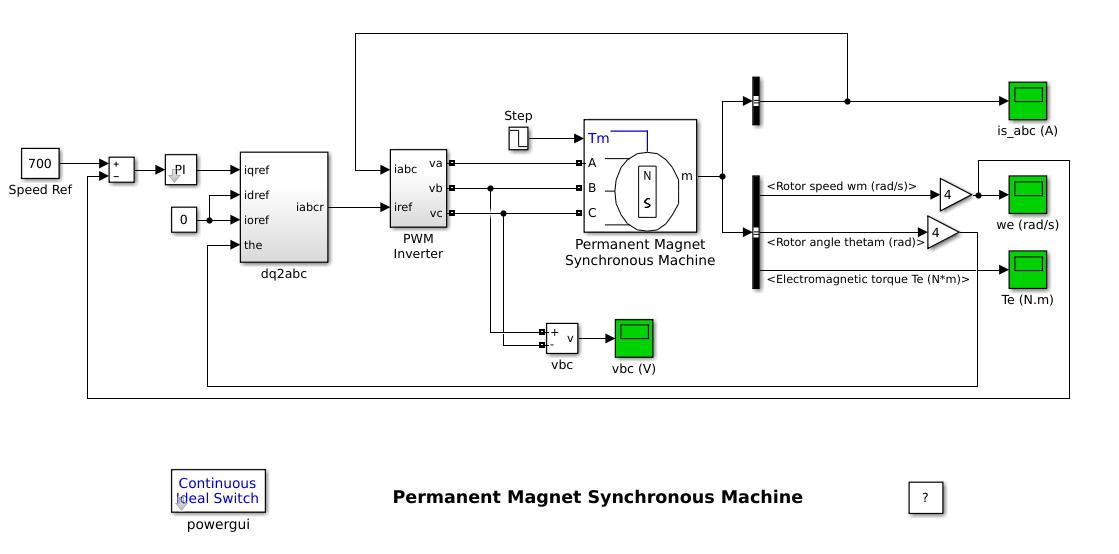
\includegraphics[width=0.8\textwidth]{./sim/pictures/powerPmmotor.png}
	\caption{power\_pmmotor Simulink Modell}
	\label{FigPowerPmmotor}
\end{figure}

zu sehen. Hier ist zu erkennen, dass in diesem Modell sowohl der Motor als auch die Sensorik (Hall-Sensoren) bereits umgesetzt sind. 

Das Modell bietet Einstellmöglichkeiten für folgende (in der Motorspezifikation angegebenen) Parameter des echten Motors sowie der Regelung:
\begin{itemize}
	\item Anzahl Polpaare
	\item Anzahl der Spulen
	\item Spulen Ansteuerungsform (sinusförmig)
	\item Rotor Typ (rund)
	\item Parameter für Modus (Generator- oder Motor-Betrieb)
	\item Spulen-Widerstand (0,33$\Omega$) 
	\item Drehmomentkonstante (0,065$Nm/A$)
	\item (Regelungsparameter): Motor-Regelung auf Drehzahl-Sollwert 
	\item P- und I-Anteil des Drehzahl-Reglers
\end{itemize}

Das Modell berechnet zusätzlich zur Drehzahl-Regelung das Motor-Drehmoment, die Werte der Hallsensoren sowie die Ströme in den Spulen. Des weiteren führt das Modell auch die Kommutierung durch, welche benötigt wird um das Drehmoment auf einem konstanten Level zu halten.

Im ersten Simulations-Modell wird also Simulink mit dem Modell \textit{power\_pmmotor} verwendet und per \textit{Virtual Serial Port Driver} an eine GUI angebunden (Implementierung des Kommunikations-Protokolls im Simulations-Kontext fehlt noch, der externe Kommunikationspartner wurde im Rahmen weiterer Teilgebiete dieses Projekts erstellt).


\section{Entwurfsphase und Implementierung I - Anpass-Arbeiten}
Es wurde damit begonnen, das Modell an den echten/geplanten Versuchsaufbau anzupassen:  
\begin{itemize}
	\item Um sich möglichst viele Freiheiten bei der Drehzahlregelung offen halten zu können, wurde geplant, einen PID-Regler zu verwenden. 
	\item Weiterhin wurden die zusätzlich benötigten Simulink-Blöcke für die serielle Kommunikation implementiert und passend parametrisiert. Da das Modell mit einem \textit{Solver} mit variabler Schrittgröße berechnet wird (hierbei berechnet der Lösungsalgorithmus von Simulink selbst, zu welchen Zeitpunkten die nächste Berechnung durchgeführt werden muss), konnte die Kommunikation nicht direkt umgesetzt werden, da die Kommunikationsblöcke nur mit \textit{Solvern} funktionieren die eine feste Schrittgröße (festes Abtastraster) verwenden. 
	Um dieses Problem zu lösen wurde hierfür ein \textit{Sample and Hold} Block eingesetzt. Dieser Block behält den Wert am Eingang so lange gültig, bis ein neuer Wert em Eingang anliegt, gibt am Ausgang jedoch zu definierten Zeiten einen Wert aus. Hiermit war es möglich zyklisch Daten aus dem Simulink Modell heraus zu senden und zu empfangen.
	\item Anschließend wurde äquivalent zum realen Versuchs-Aufbau begonnen Protobuff %todo: namen checken
	zu implementieren, da die GUI-Schnittstelle mit diesem Protokoll kommuniziert. Diese Arbeiten wurde dann zugunsten eines alternativen Motormodells (s.u.) allerdings auf Eis gelegt.
\end{itemize}


\section{Analysephase II - Alternativ-Modell}
Da ohne den echten Aufbau nicht weiter getestet werden konnte, ob das in der ersten Entwurfsphase ausgewählte Matlab Modell den Aufbau bereits ausreichend genau beschreiben kann und zum anderen die Komplexität dieses Modells sehr hoch ist, wurde beschlossen, ein neues, eigenes und nach Möglichkeit einfacheres Alternativ-Modell zu erstellen.


\section{Entwurfsphase II - eigene Motor-Modellierung}
Das Alternativ-Modell für den Motor sollte folgende Form haben - siehe Abbildung \ref{FigMotorBlock}:

\begin{figure}[htbp]
	\centering
	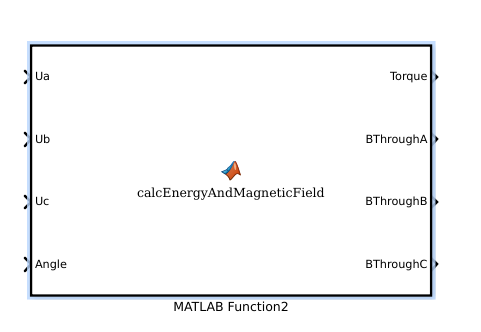
\includegraphics[width=0.6\textwidth]{./sim/pictures/matlabBox.png}
	\caption{Eigenschaften neuer Simulink Motor Block}
	\label{FigMotorBlock}
\end{figure}
Hierbei sind die Eingangsgrößen zu erkennen
\begin{itemize}
	\item $U_a$, $U_b$, $U_c$ an den drei Phasen U/V/W (an Spulen anliegende Spannung)
	\item Angle (Drehwinkel)
\end{itemize}
sowie die Ausgangsgrößen
\begin{itemize}
	\item \textit{BThroughA}, \textit{BThrougB} und \textit{BThrougC} (Spulen durchdringendes Magnetfeld)
	\item \textit{Torque} (Drehmoment)
\end{itemize}

\vspace{1cm}
Der Motor ist wie in Abbildung \ref{FigMotorAufbau} zu sehen ist aufgebaut:

\begin{figure}[htbp] 
	\centering
	\includestandalone{./sim/pictures/motorAufbau}
	\caption{Motor Aufbau}
	\label{FigMotorAufbau}
\end{figure}


Hierbei sind die 14 Permanentmagneten im außen laufenden Rotor zu erkennen. Diese sind so angeordnet, dass sich ihre Polung kontinuierlich abwechselt. 

Im Inneren des Motors sind die einzelnen Spulen des Stators zu erkennen. Mithilfe der farbigen Zuordnung ist es möglich zu identifizieren welche Spulen zu einer großen Spule (U,V oder W) zusammengeschlossen sind. 

Es ist zu erkennen, dass die großen Spulen sternförmig (über die Teil-Spulen 4, 5 und 12) zusammengeschaltet sind (der Sternpunkt des Motors ist von außen nicht zugänglich).
Die U/V/W-Anschlüsse sind mithilfe der Pfeile markiert (vgl. Spule 1, 8 und 9). 
Es sollte noch erwähnt werden, dass die Spulen unterschiedlich gewickelt sind. So sind die Spulen 1, 3, 6, 8, 9 und 11 im Uhrzeigersinn gewickelt und die Spulen 2, 4, 5, 7, 10 und 12 entgegen diesem.

In der symbolischen Abbildung ist zu erkennen, dass sowohl zwischen den Permanentmagneten im Rotor, als auch zwischen den Spulen im Stator jeweils Abstände existieren. 
Im realen Motor ist außerdem ein Luftspalt zwischen dem Rotor und dem Stator vorhanden. 
Die Formgebung der Polschuhe wird nicht dargestellt.


Vereinfachungs-Annahmen: 
Da ein einfaches Modell erstellt werden sollte, wurden folgende Annahmen getroffen, vgl. auch Abbildung \ref{FigVereinfachtesModell}:
\begin{itemize}
	\item Zwei der drei Phasen werden in der Darstellung mit Spannung versorgt, die dritte Spule ist offen.
	\item Alle Luftspalte werden vernachlässigt. D.h. weder die räumlichen Abstände zwischen den Permanentmagneten im Rotor noch der räumliche Verlauf der von den Spulen in Stator erzeugten Magnetfelder werden modelliert. 
	\item Weiterhin wird insbesondere auch der Luftspalt zwischen Rotor und Stator vernachlässigt.
	\item Es werden nur senkrechte Magnetfeldlinien angenommen, der Einfluss der Polschuhe wird vernachlässigt.
	\item Die Zuordnung der Spulen zu den großen Spulen, die Verbindung mit den Zuleitungen usw. entspricht der vorhergehenden Abbildung. 
\end{itemize}

\begin{figure}[htbp]
	\begin{center}
		\includestandalone{./sim/pictures/vereinfachtesModell}
		\caption{Vereinfachtes Modell}
		\label{FigVereinfachtesModell}
	\end{center}
	
\end{figure}


Um dieses Modell mithilfe von Arrays in Simulink umsetzen zu können, wurde gedanklich zwischen 1 und 12/14 aufgeschnitten und der Kreis ausgerollt. Dabei ergibt sich dann folgendes Bild \ref{FigAbgerolltesModell}.


\begin{figure}[htbp]
	\begin{center}
		\includestandalone{./sim/pictures/abgerolltesModell}
		\caption{Abgerolltes Modell}
		\label{FigAbgerolltesModell}
	\end{center}
	
\end{figure}

%\FloatBarrier
\section{Implementierung II - neues Motormodell}
Für die genaue Modellierung wurde folgender Ansatz verwendet: Sowohl für den Stator als auch den Rotor wird ein Array angelegt. Beim Rotor (Permanentmagnete) werden die Einträge mithilfe einer Konstanten für die magnetische Flussdichte gefüllt, dabei bekommt jeder Nordpol willkürlich gewählt ein positives und jeder Südpol ein negatives Vorzeichen. 

Da (wie im Bild zu erkennen ist) der Rotor 14 und der Stator zwölf Einheiten besitzen, wird die Anzahl der Arrayeinträge auf (mindestens) das kleinste gemeinsame Vielfache (84) festgelegt. Somit ist es mithilfe des Modells möglich den Motor simuliert in 84 Stufen zu drehen was einer Schrittgröße von ca. 4,3$^{\circ}$ entspricht. 

Für das Array des Stators wird berücksichtigt, welche Spulen aktuell bestromt sind und wie groß die angelegte Spannung ist. Mit Hilfe der Spannung und dem Spulen-Widerstand kann eine statische Stromstärke berechnet werden (die Induktivität der Spulen wird zunächst vernachlässigt), daraus lässt sich die magnetische Flussdichte in den Spulen bestimmen. 

Abhängig vom Winkel und der angelegten Spannung (d.h. welche Spulen bestromt sind) wird das Array für den Stator entsprechend befüllt. 

Anschließend wird abhängig vom Winkel das Rotor Array rotiert. 

Das resultierende Magnetfeld wird bestimmt, indem diejenigen Array-Einträge addiert werden, die sich einander gegenüber befinden. 
Die Einträge des so entstanden resultierenden Arrays werden quadriert (und durch die Konstante $2*\mu_0$ geteilt). 

Um am Ende die Energie zu errechnen, welche zu diesem Zeitpunkt im resultierenden Magnetfeld steckt, wird über die einzelnen Array-Einträge integriert. 
Somit ergibt sich ein Energiewert für diesen Zustand bzw. Zeitpunkt. 

Um das resultierende Drehmoment zu erhalten wird dieselbe Rechnung erneut durchgeführt, allerdings für den Fall, dass der Rotor $1/84$ weiter gedreht wird. 

Aus der Differenz dieser beiden Energiewerte kann das Drehmoment bestimmt werden unter der Annahme, dass die ganze Energie-Änderung in die Beschleunigung des Rotors eingeht.

Zusätzlich werden die resultierenden Magnetfelder über den Spulen (U,V und W) ebenfalls aufintegriert, um mit Hilfe dieser Werte im weiteren Modellaufbau die Induktionsspannung berechnen zu können.

\section{Bewertung des neuen Modells}
Bei der Untersuchung des neuen Modells muss festgehalten werden, dass die Induktivität der Spulen nicht mithilfe dieses Modells berechnet werden kann. 
Der modellierte Magnetfeld-Verlauf für eine Spule hat die in Abbildung \ref{FigResultierendesFeld}
dargestellte Form.

\begin{figure}[htbp]
	\centering
	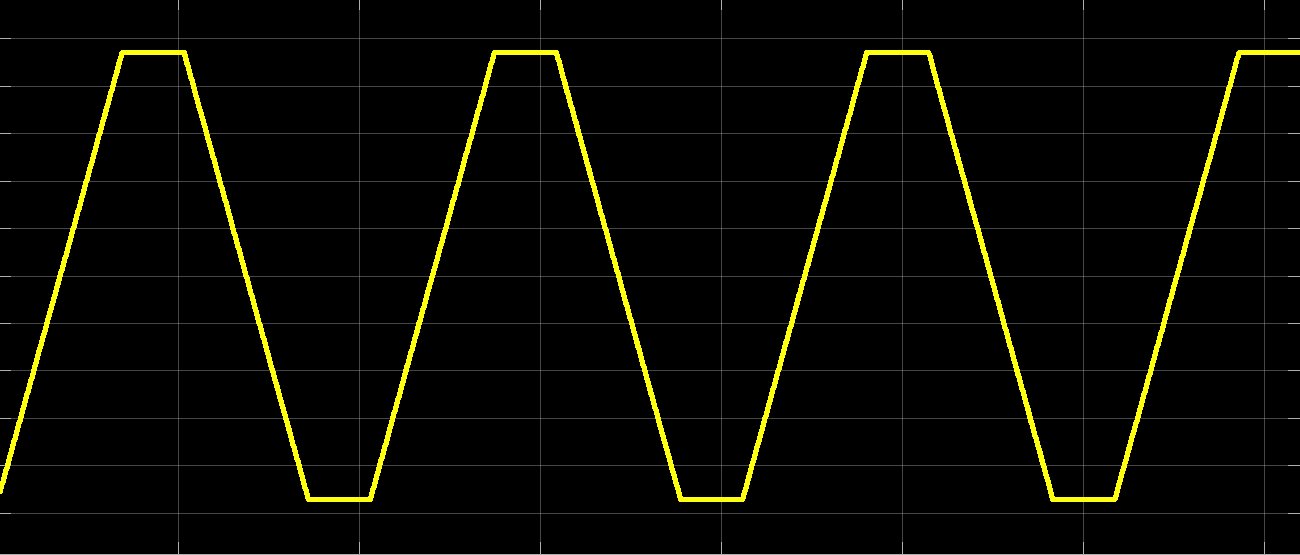
\includegraphics[width=0.8\textwidth]{./sim/pictures/resultierendesFeld.png}
	\caption{Verlauf Magnetfeld in einer Spule}
	\label{FigResultierendesFeld}
\end{figure}

Dies lässt sich dadurch begründen, dass bei der Betrachtung einer Spule (z.B. der V-Spule) für das Feld im Stator 4*7= 28 Array-Elemente des resultierenden Arrays beteiligt sind. Über diese wird integriert, um die Größe für das Feld zu bekommen, was einer Aufsummierung der beteiligten Array-Elemente entspricht $\sum \limits_1^{28} V_{res_i}$. 

Wobei sich ein Eintrag $V_{res_i}$ aus der Addition des Spuleneintrags $V_i$ und des Eintrags des darüber liegenden $R_i$ also dem Wert des Rotormagnetfeldes an dieser Stelle ergibt. So lässt sich $\sum \limits_1^{28} V_{res_i}$ zu $\sum \limits_1^{28} (V_i+R_i)$ umstellen. Diese Summe lässt sich nun allerdings nun in zwei Summen zerlegen, zum einen in $\sum \limits_1^{28} V_i$ und zum anderen $\sum \limits_1^{28} R_i$. 

Hierbei ist die erste Summe  $\sum \limits_1^{28} V_i$ immer 0, da die vier Spulen einer großen Spule (im Beispiel Phase V) in der Wicklungsrichtung abwechseln. 

Somit bleibt nur noch $\sum \limits_1^{28} R_i$ übrig um den Verlauf zu erklären: Wie in Abbildung \ref{FigAbgerolltesModell} zu erkennen ist, ist ein Element des Rotors kleiner als eines des Stators. So kürzen sich zwar auch viele Elemente des Rotors heraus, jedoch nicht alle. Dies führt zum erkennbaren Magnetfeld-Verlauf. 

Das hat jedoch nicht wirklich etwas mit dem Verlauf zu tun, der modelliert werden soll. Aus diesem Grund ist das Modell hierfür nicht passend und sollte nicht ohne weitere Änderungen verwendet werden (insbesondere bedeutet eine ausschließlich statische Betrachtung der Magnetfeldverläufe eine unzulässige Vereinfachung).

Hingegen scheint der Verlauf für das Drehmoment durchaus Sinn zu ergeben, wie in Abbildung \ref{FigDrehmoment} zu erkennen ist: Da in diesem Modell in die Berechnung der resultierenden  Energie ein Quadrat eingeht, ist hier das zuvor beschriebene Verhalten des Wegkürzens nicht mehr vorhanden. 

Es ist jedoch noch darauf hinzuweisen, dass eine Vergrößerung der Anzahl an Array-Elementen (entspricht einer Erhöhung der Auflösung) nicht dazu führt, dass dieser Verlauf glatter werden würde, sondern es werden immer dieselben zwölf Stufen, welche den Spulen-Polpaaren entsprechen, im Verlauf zu erkennen sein.
Dies ist eine Folge der zu Beginn getroffenen Vereinfachungen, wonach Luftspalt, Polform und nicht-senkrechte Magnetfeldlinien vernachlässigt wurden.


\begin{figure}[htbp]
	\centering
	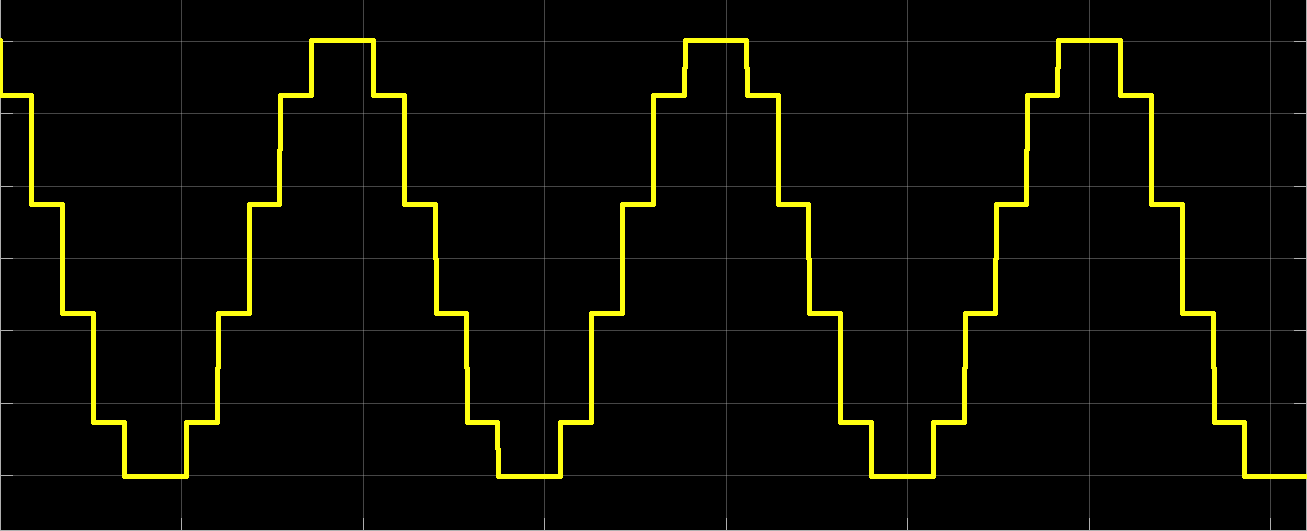
\includegraphics[width=0.8\textwidth]{./sim/pictures/drehmoment.png}
	\caption{Drehmoment bei Spannung an $U_a$ und Masse bei $U_b$}
	\label{FigDrehmoment}
\end{figure}


\section{Bewertung der beiden Modelle}
Für eine Simulation des Motor-Experimentierplatzes ist das zweite Modell (zumindest in der vorliegenden Form) nicht geeignet, es geht von statischen Zuständen aus und vernachlässigt die dominanten Parameter (Induktivität, Luftspaltgestaltung usw.) eines realen Motors.

Ein Vergleich des ersten Modells mit dem Verhalten des realen Experimentierplatzes steht noch aus.

\section{Ausblick}
Für das neue, zweite Modell gibt es noch viel Verbesserungs-Potenzial, z.B.:

\begin{itemize}
	\item So wäre es möglich, bzw. wurde schon damit begonnen, die Kommutierung umzusetzen. Diese soll anhand des Winkels die Spulen unterschiedlich an Masse und Spannung anschließen mit dem Ziel ein konstantes Drehmoment zu erhalten.
	
	\item Mit dieser Erweiterung könnte dann ein (Strom-/Drehmoment-)Regler implementiert werden welcher z.B. auf ein konstantes Drehmoment regelt.
	
	\item Das reale Drehmoment ist eine Funktion zahlreicher mechanischer und elektromagnetischer Details der Motorgestaltung. Einfluss der Induktivität, Luftspaltgestaltung usw. könnten Gegenstand weiterer Modell-Verfeinerungen sein. 
	
	\item Um das neue Modell in die Simulationsumgebung anstelle des ersten Modells einbetten zu können, sind dieselben Erweiterungen durchzuführen, mit denen bereits am ursprünglichen Modell begonnen wurde (z.B. damit auch dieses Modell in der Lage wäre mit der GUI zu kommunizieren, um simulierte Größen auszutauschen bzw. von dort Regelgrößen zu bekommen).
\end{itemize}

Zuvor sollte das erste Modell (Matlab-Bausteine) weiter mit dem Verhalten des realen Motor-Experimentierplatzes verglichen werden (Messwerte). 

Da der reale Aufbau noch nicht fertiggestellt war, konnte hierfür noch keine eindeutige Modell-Bewertung gegeben werden.




